\section{Desarrollo}

\subsection*{Parte 1: Madurez}

En primer lugar se determina la madurez del hormigón según el método de Plowman, para luego determinar el tiempo necesario para alcanzar la resistencia requerida con los metodos de Nurse-Saul como la de Freieslaben, Hansen y Pedersen.

\subsubsection*{Plowman}

Considerando una temperatura de terreno de 23 °C ($T_r$), asi como $T_D$ tiene un valor de 0 °C, se calcula la madurez como:

\begin{equation}
    M = t_{eq} (T_r - T_D) \quad \text{donde} \quad t_{eq} = 13.27
\end{equation}

A partir de los datos entregados, se obtiene la siguiente tabla:

\begin{table}[H]
\centering
\renewcommand{\arraystretch}{1.15}
\begin{tabular}{r r r r r r r r}
\hline
\multicolumn{1}{c}{Edad} & \multicolumn{1}{c}{Temperatura} & \multicolumn{1}{c}{Resistencia} & \multicolumn{1}{c}{dt} & \multicolumn{1}{c}{T prom} & \multicolumn{1}{c}{Madurez} & \multicolumn{1}{c}{Madurez} & \multicolumn{1}{c}{Plowman} \\
\multicolumn{1}{c}{[días]} & \multicolumn{1}{c}{[°C]} & \multicolumn{1}{c}{MPa} & \multicolumn{1}{c}{días} & \multicolumn{1}{c}{C} & \multicolumn{1}{c}{C*h} & \multicolumn{1}{c}{C*dia} & \multicolumn{1}{c}{C*hr} \\
\hline
0 & 29 & 0 & 0 & -- & 0 & 0 & 0 \\
0.25 & 39 & 0.39 & 0.25 & 34 & 8.5 & 7 & 168 \\
0.5 & 49 & 0.88 & 0.25 & 44 & 19.5 & 14 & 336 \\
0.75 & 54 & 1.42 & 0.25 & 51.5 & 32.375 & 21 & 504 \\
1 & 59 & 2.01 & 0.25 & 56.5 & 46.5 & 28 & 672 \\
1.5 & 64 & 3.29 & 0.5 & 61.5 & 77.25 & 42 & 1008 \\
2 & 59 & 4.47 & 0.5 & 61.5 & 108 & 56 & 1344 \\
2.5 & 48 & 5.43 & 0.5 & 53.5 & 134.75 & 70 & 1680 \\
3 & 44 & 6.31 & 0.5 & 46 & 157.75 & 84 & 2016 \\
3.5 & 39 & 7.09 & 0.5 & 41.5 & 178.5 & 98 & 2352 \\
4 & 34 & 7.77 & 0.5 & 36.5 & 196.75 & 112 & 2688 \\
4.5 & 29 & 8.35 & 0.5 & 31.5 & 212.5 & 126 & 3024 \\
5 & 26 & 8.87 & 0.5 & 27.5 & 226.25 & 140 & 3360 \\
5.5 & 26 & 9.39 & 0.5 & 26 & 239.25 & 154 & 3696 \\
6 & 23 & 9.85 & 0.5 & 24.5 & 251.5 & 168 & 4032 \\
7 & 23 & 10.77 & 1 & 23 & 274.5 & 196 & 4704 \\
8 & 23 & 11.69 & 1 & 23 & 297.5 & 224 & 5376 \\
9 & 23 & 12.61 & 1 & 23 & 320.5 & 252 & 6048 \\
10 & 23 & 13.53 & 1 & 23 & 343.5 & 280 & 6720 \\
11 & 23 & 14.45 & 1 & 23 & 366.5 & 308 & 7392 \\
14 & 23 & 17.21 & 3 & 23 & 435.5 & 392 & 9408 \\
21 & 23 & 23.65 & 7 & 23 & 596.5 & 588 & 14112 \\
28 & 23 & 30.09 & 7 & 23 & 757.5 & 784 & 18816 \\
\hline
\end{tabular}
\end{table}

De esta manera, interpolando la madurez obtenida, se obtiene un tiempo de 8.33 dias, es decir, ese es el tiempo nesesario para el hormigon en obra tenga una resitencia similar a la resitencia alcanzada a los 13.27 dias en laboratorio.

Ahora, es nesesario determinar a madurez del hormigon al $85\%$ de $f_{cm}$, donde considerando un hormigon G20 con 4MPa de desviacion estandar, se obtiene:

\begin{equation}
    0.85 \cdot f_{cm} = f'_c + t \cdot s = (20 + 1.282 \cdot 4)\cdot 0.85 = 21.35 MPa
\end{equation}

Luego se obtienen los factores K1 y K2 a partir de los valores de 3 y 28 dias:

\begin{equation}
    6.31 = K_1 + K_2 log(2016)
\end{equation}

\begin{equation}
    30.09 = K_1 + K_2 log(18816)
\end{equation}

De esta forma, $K_1 = -74.698$ y $K_2 = 24.514$. Luego, la madurez para la resitencia requerida es:

\begin{equation}
    R(M) = K_1 + K_2 log(M)
\end{equation}

\begin{equation}
    21.35 = -74.698 + 24.514 log(M)
\end{equation}

De esta forma, la madurez requerida es de $M = 345.264$ C dia.

\subsubsection*{Nurse-Saul}

El metodo establece que el tiempo equivalente se puede calcular como:

\begin{equation}
    \Delta t_{eq} = \frac{T_i - T_d}{T_r - T_d} \Delta t_i
\end{equation}

De esta forma, se obtiene la siguiente tabla:

\begin{table}[H]
\centering
\renewcommand{\arraystretch}{1.15}
\begin{tabular}{r r r r r}
\hline
\multicolumn{1}{c}{Edad [días]} & \multicolumn{1}{c}{Temperatura [°C]} & \multicolumn{1}{c}{t eqi obra [días]} & \multicolumn{1}{c}{t equi lab [días]} & \multicolumn{1}{c}{Madurez c dia} \\
\hline
0 & 29 & 0 & 0 & 0 \\
0.25 & 39 & 0.423913043 & 0.39 & 7 \\
0.5 & 49 & 0.956521739 & 0.88 & 14 \\
0.75 & 54 & 1.543478261 & 1.42 & 21 \\
1 & 59 & 2.184782609 & 2.01 & 28 \\
1.5 & 64 & 3.576086957 & 3.29 & 42 \\
2 & 59 & 4.858695652 & 4.47 & 56 \\
2.5 & 48 & 5.902173913 & 5.43 & 70 \\
3 & 44 & 6.858695652 & 6.31 & 84 \\
3.5 & 39 & 7.706521739 & 7.09 & 98 \\
4 & 34 & 8.445652174 & 7.77 & 112 \\
4.5 & 29 & 9.076086957 & 8.35 & 126 \\
5 & 26 & 9.641304348 & 8.87 & 140 \\
5.5 & 26 & 10.20652174 & 9.39 & 154 \\
6 & 23 & 10.70652174 & 9.85 & 168 \\
7 & 23 & 11.70652174 & 10.77 & 196 \\
8 & 23 & 12.70652174 & 11.69 & 224 \\
9 & 23 & 13.70652174 & 12.61 & 252 \\
10 & 23 & 14.70652174 & 13.53 & 280 \\
11 & 23 & 15.70652174 & 14.45 & 308 \\
14 & 23 & 18.70652174 & 17.21 & 392 \\
21 & 23 & 25.70652174 & 23.65 & 588 \\
28 & 23 & 32.70652174 & 30.09 & 784 \\
\hline
\end{tabular}
\end{table}

Luego, interpolando la madurez obtenida, se obtiene un tiempo de 17.037 dias en obra y 15.674 dias en laboratorio para alcanzar la resitencia requerida de 21.35 MPa.

\subsection*{Freiesleben Hansen y Pedersen}

El metodo establece que el tiempo equivalente se puede calcular como:

\begin{equation}
    t_{eq} = \sum e^{-Q \cdot (\frac{1}{T_a} - \frac{1}{T_s})} \Delta t_i
\end{equation}

Donde Q corresponde a la energia de activacion, para cemento tipo I Q = 5000. Por simplicidad, se considerara que para cemento tipo II Q no varia.. De esta forma, se obtiene la siguiente tabla:

\begin{table}[H]
\centering
\renewcommand{\arraystretch}{1.15}
\begin{tabular}{r r r r r r}
\hline
\multicolumn{1}{c}{Edad} & \multicolumn{1}{c}{Temperatura} & \multicolumn{1}{c}{Madurez} & \multicolumn{1}{c}{K prom} & \multicolumn{1}{c}{teq obra} & \multicolumn{1}{c}{teq lab} \\
\hline
0 & 29 & 0 & 273.15 & 0 & 0 \\
0.25 & 39 & 7 & 307.15 & 0.457650536 & 0.40864708 \\
0.5 & 49 & 14 & 317.15 & 1.222276193 & 1.091399566 \\
0.75 & 54 & 21 & 324.65 & 2.322859691 & 2.074136823 \\
1 & 59 & 28 & 329.65 & 3.713048795 & 3.315469833 \\
1.5 & 64 & 42 & 334.65 & 7.200620997 & 6.429606238 \\
2 & 59 & 56 & 334.65 & 10.6881932 & 9.543742643 \\
2.5 & 48 & 70 & 326.65 & 13.10702707 & 11.7035771 \\
3 & 44 & 84 & 319.15 & 14.79507793 & 13.21087797 \\
3.5 & 39 & 98 & 314.65 & 16.14428463 & 14.41561682 \\
4 & 34 & 112 & 309.65 & 17.1881452 & 15.34770482 \\
4.5 & 29 & 126 & 304.65 & 17.98899055 & 16.06279874 \\
5 & 26 & 140 & 300.65 & 18.63274066 & 16.63761856 \\
5.5 & 26 & 154 & 299.15 & 19.22498612 & 17.16644866 \\
6 & 23 & 168 & 297.65 & 19.76938993 & 17.65255981 \\
7 & 23 & 196 & 296.15 & 20.76938993 & 18.54548366 \\
8 & 23 & 224 & 296.15 & 21.76938993 & 19.43840751 \\
9 & 23 & 252 & 296.15 & 22.76938993 & 20.33133136 \\
10 & 23 & 280 & 296.15 & 23.76938993 & 21.22425522 \\
11 & 23 & 308 & 296.15 & 24.76938993 & 22.11717907 \\
14 & 23 & 392 & 296.15 & 27.76938993 & 24.79595062 \\
21 & 23 & 588 & 296.15 & 34.76938993 & 31.04641759 \\
28 & 23 & 784 & 296.15 & 41.76938993 & 37.29688455 \\
\hline
\end{tabular}
\end{table}

Luego, interpolando la madurez obtenida, se obtiene un tiempo de 26.100 dias en obra y 23.305 dias en laboratorio para alcanzar la resitencia requerida de 21.35 MPa.

Las razones en la diferencia de cada metodo radica en que el modelo Nurse-Saul es un modelo mas simple y lineal, que no considera los efectos de la reaccion. En cambio, el modelo de Freiesleben Hansen y Pedersen considera la energia de activacion y la variacion de la temperatura, en un modelo exponencial, lo que lo hace mas preciso para predecir la resistencia del hormigon en funcion del tiempo y la temperatura. Ahora bien, la energia de activacion en este ultimo metodo juega un roll fundamental, donde se observa que a valores mayores, el tiempo equivalente aumenta, lo cual se traduce en que la reaccion ocurre mas lento.

\subsection*{Parte 2: Presion de Moldajes}

Se tienen los siguientes datos de entrada:

\begin{table}[H]
\centering
\renewcommand{\arraystretch}{1.2}
\begin{tabular}{c c c c c c}
\hline
\begin{tabular}{@{}c@{}}Tipo\\ de Cemento\end{tabular} &
\begin{tabular}{@{}c@{}}Cono de\\ Asentamiento (mm)\end{tabular} &
\begin{tabular}{@{}c@{}}Densidad\\ (kg/m\textsuperscript{3})\end{tabular} &
\begin{tabular}{@{}c@{}}Altura de\\ Colocación (m)\end{tabular} &
\begin{tabular}{@{}c@{}}Temperatura\\ ($^\circ$C)\end{tabular} &
\begin{tabular}{@{}c@{}}Presión\\ Lateral (kPa)\end{tabular} \\
\hline
II & 148 & 2376 & 6.1 & 16.4 & 89 \\
\hline
\end{tabular}
\end{table}

Los cuales fueron ingresados en la calculadora de presión de moldajes de la página \href{https://apps.peri.com/SLR/index.php?lang=en&norm=aci}{PERI}. Los datos fueron ingresados como se muestra en la siguiente imagen:

\begin{figure}[H]
    \centering
    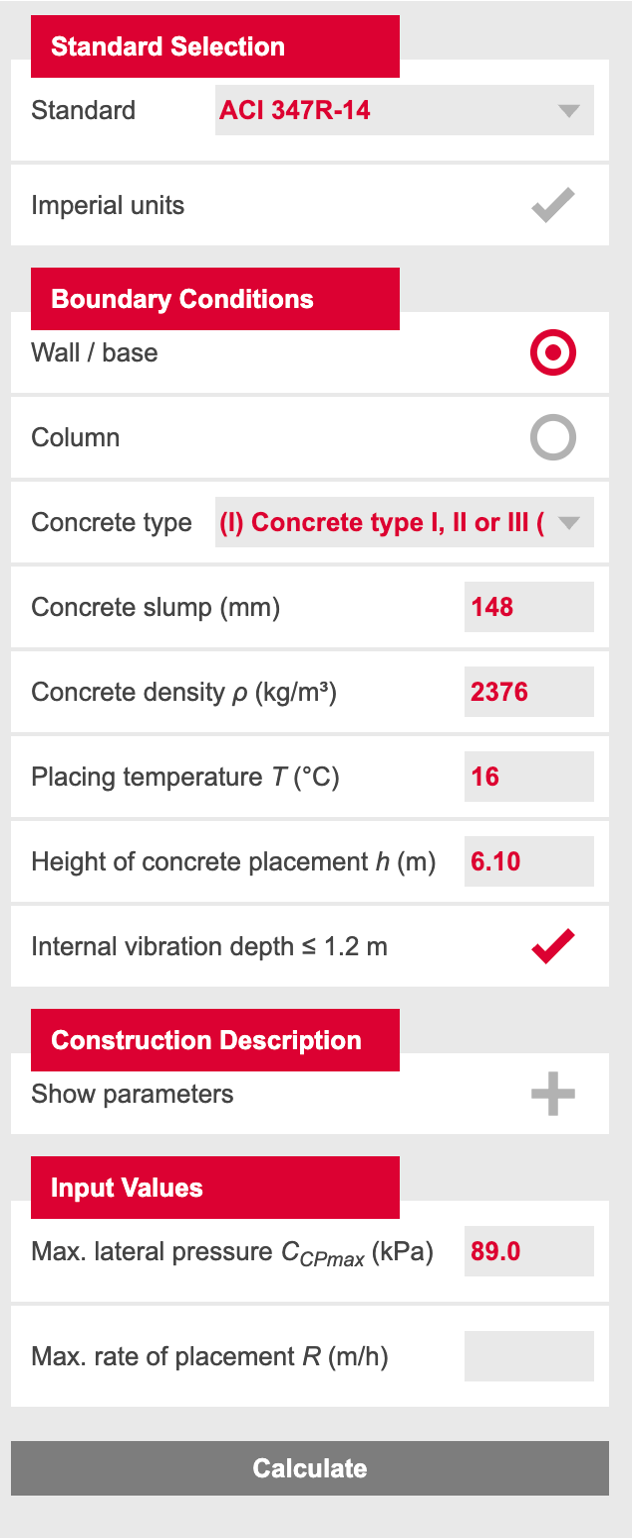
\includegraphics[width=0.5\linewidth]{datos_entrada.png}
    \caption{Datos ingresados en la calculadora de PERI}
\end{figure}

Lo cual da el siguiente resultado:

\begin{figure}[H]
    \centering
    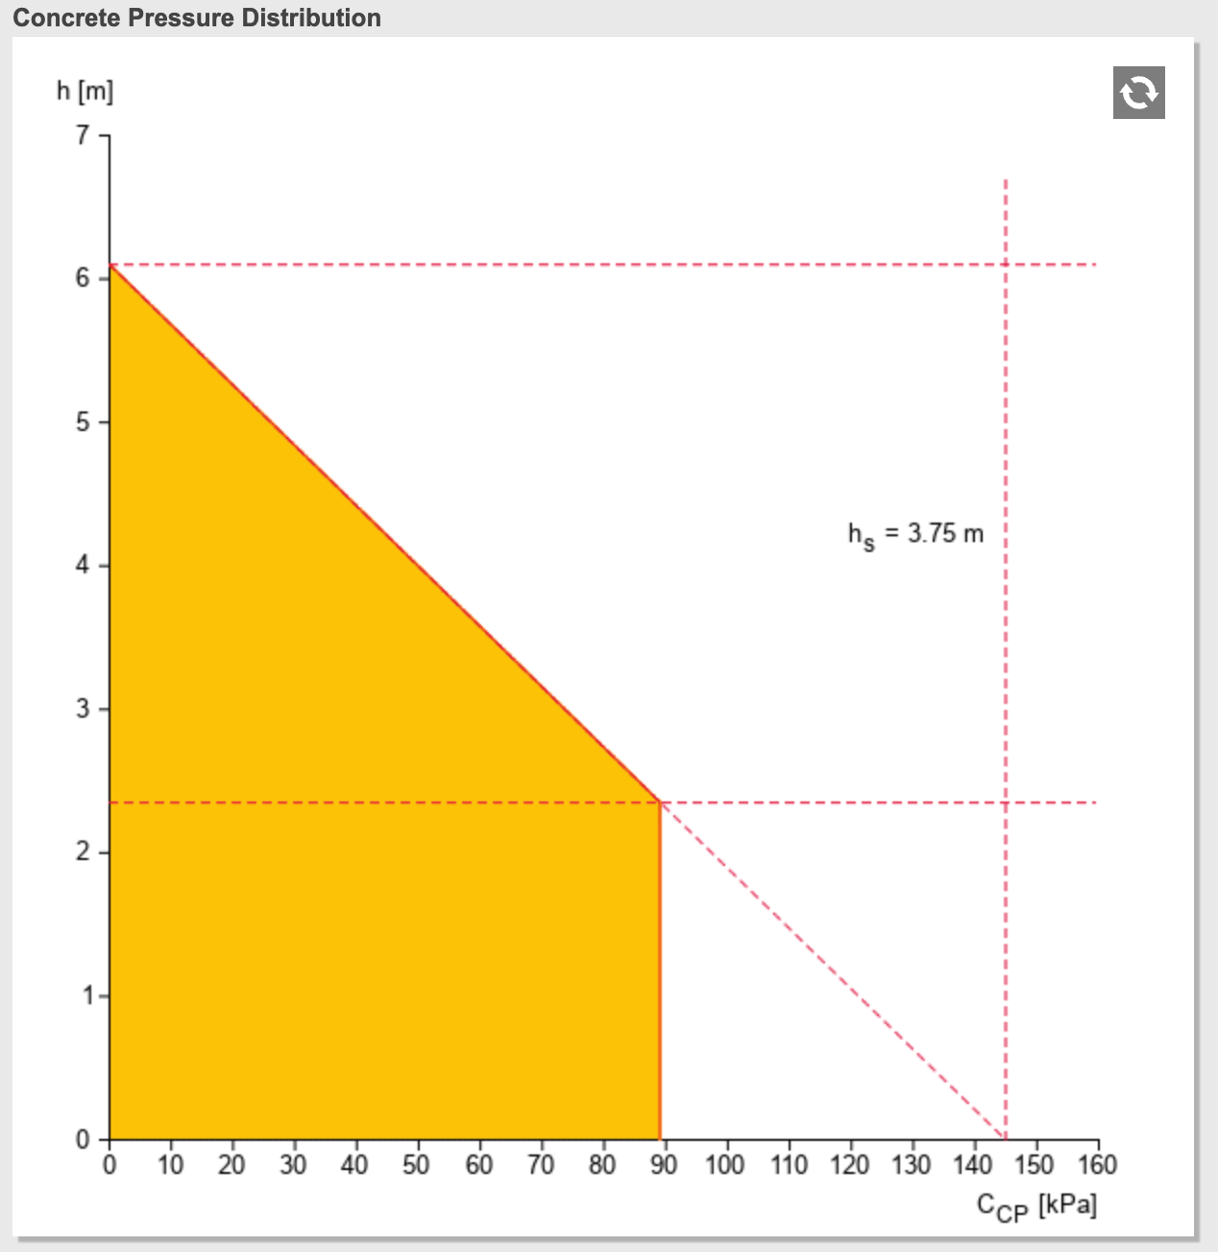
\includegraphics[width=0.5\linewidth]{resultado.png}
    \caption{Resultado de la calculadora de PERI}
\end{figure}

Donde no se genera un limite del hormigonado, por lo tanto, se puede realizar la solicitud de 10 $m/h$ sin problemas.

Ahora bien, si la presion maxima es un 80\% de la presion indicada, es decir, 71.2 kPa, para mantener el rendimiento de 10 $m/h$, se propone disminuir la densidad del hormigon a 2150 kg/m$^3$. Ingresando este nuevo valor en la calculadora, se obtiene el siguiente resultado:

\begin{figure}[H]
    \centering
    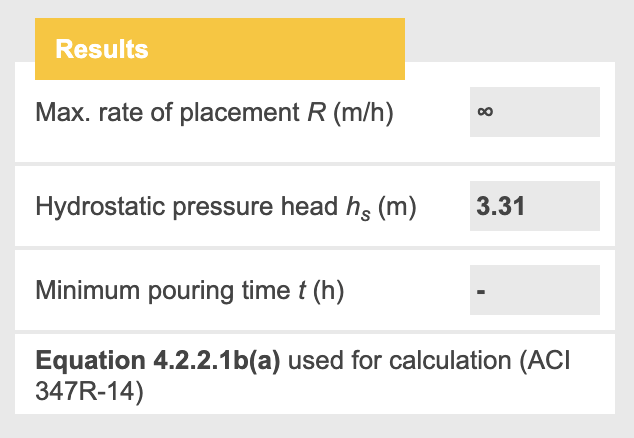
\includegraphics[width=0.5\linewidth]{max_rate.png}
    \caption{Resultado de la calculadora de PERI con densidad reducida}
\end{figure}

Donde el grafico de distribucion de presion es:

\begin{figure}[H]
    \centering
    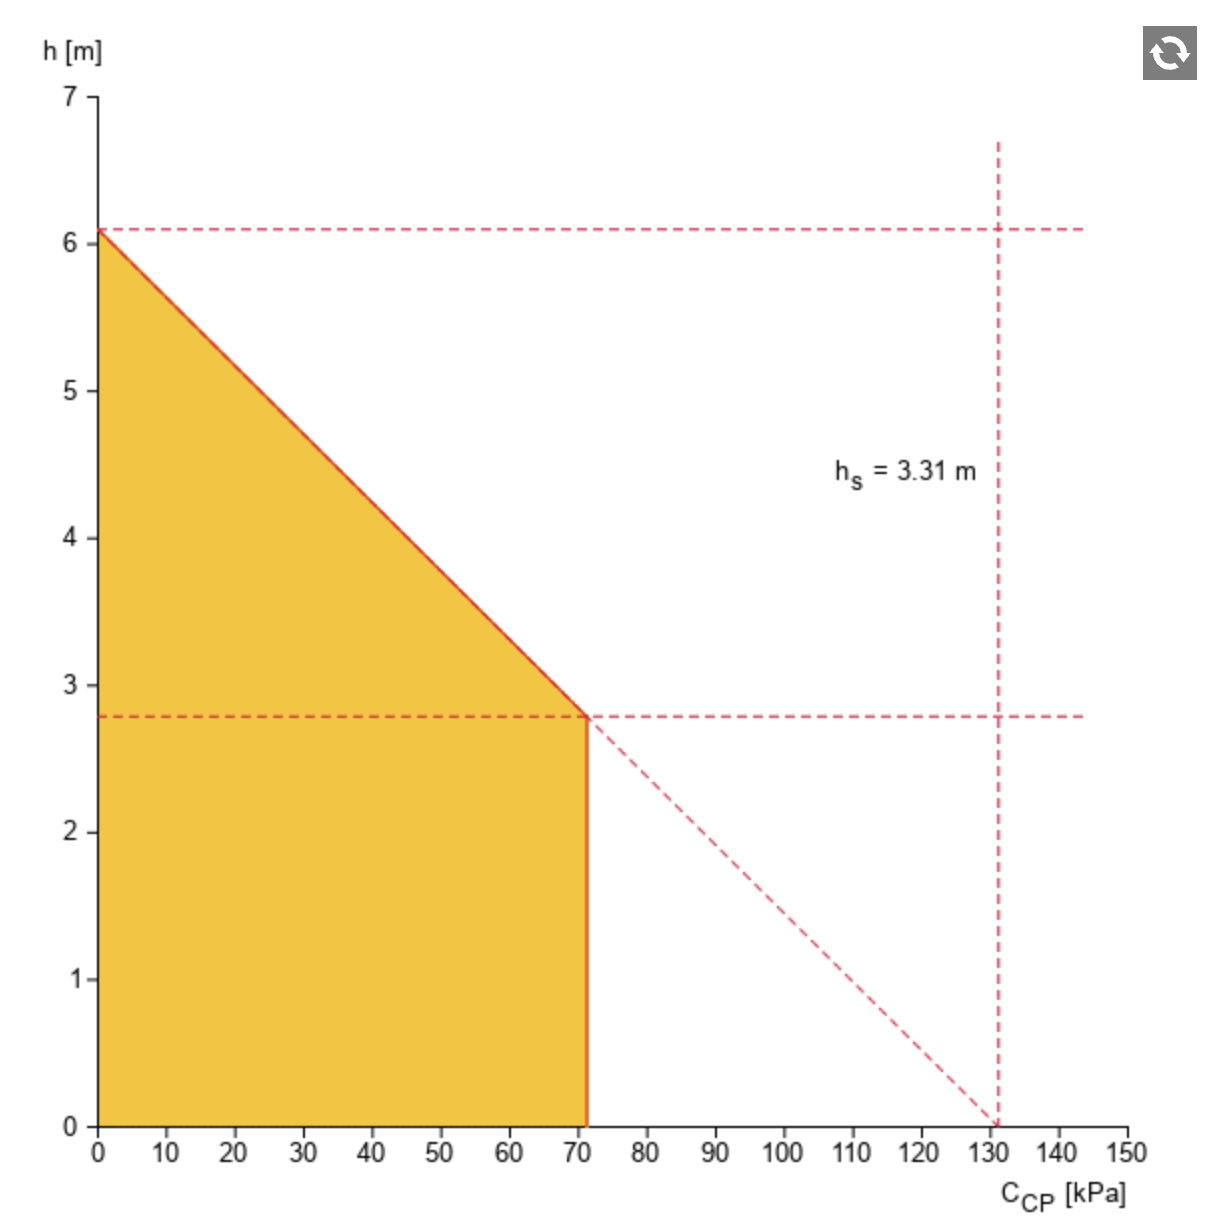
\includegraphics[width=0.5\linewidth]{presiones_2.png}
    \caption{Distribucion de presion con densidad reducida}
\end{figure}

Para lograr tal objetivo, se puede generar un hormigon con agregados livianos.

\subsection*{Parte 3: Bolomey y Venuat}

En esta parte se requirió determinar el tiempo mínimo de desmolde de una columna para optimizar el presupuesto de la obra. Se compararon los tiempos de desmimbre utilizando un hormigón tradicional con uno de alta resistencia. 
Para el desarrollo de esta sección, se utilizaron los métodos de Bolomey y Venuat, los cuales permiten estimar la resistencia del hormigón en función de su dosificación y del tiempo de curado.

A continuación, se presentan los datos utilizados, los cálculos realizados para ambos tipos de hormigón y los resultados obtenidos.

\begin{table}[H]
\centering
\caption{Datos experimentales – Grupo 5}
\renewcommand{\arraystretch}{1.15}
\small
\begin{tabular}{lccc}
\hline
%\rowcolor[HTML]{EFEFEF}
\textbf{Parámetro} & \textbf{Unidad} & \textbf{Cem. corriente} & \textbf{Cem. alta resistencia} \\ \hline
Agua utilizada & kg/m$^3$ & 166.32 & 153.68 \\
Cemento mezcla 1 (Z1 / V1) & kg/m$^3$ & 432.23 & 324.68 \\
Cemento mezcla 2 (Z2 / V2) & kg/m$^3$ & 312.42 & 381.65 \\
Resistencia 14 días mezcla 1 & MPa & 20.45 & 24.24 \\
Resistencia 14 días mezcla 2 & MPa & 15.47 & 33.20 \\
Resistencia 28 días mezcla 1 & MPa & 27.27 & 29.55 \\
Resistencia 28 días mezcla 2 & MPa & 22.42 & 43.11 \\
Agua para columnas & kg/m$^3$ & 141 & 141\\ \hline
\end{tabular}
\end{table}

\subsubsection*{Resistencia a la compresión}

En primer lugar, se determinó la resistencia requerida a partir de la especificada utilizando la siguiente fórmula: $f_{cm} = f_c + t \cdot s$, donde $f_c$ es la resistencia especificada, $t$ es un factor de seguridad y $s$ es la desviación estándar del hormigón.

\begin{table}[H]
\centering
\caption{Resistencia requerida para el desmolde}
\begin{tabular}{lcc}
\hline
Parámetro & Símbolo & Valor [MPa] \\ \hline
Desviación estándar & $s$ & 3.42 \\
Factor de seguridad & $t$ & 2.113 \\
Resistencia especificada & $f'_c$ & 28.86 \\
Resistencia requerida & $f_{cm}$ & 36.08 \\
Porcentaje requerido & \% & 90 \\
Resistencia mínima para desmolde & $f_{req}$ & 32.47 \\ \hline
\end{tabular}
\end{table}

\subsubsection*{Dosis mínima de cemento}

En segundo lugar, se utilizó el método de Bolomey para determinar la dosis de cemento a utilizar para alcanzar la resistencia requerida. Se utilizó esta fórmula $R = a(\frac{c}{w} - b)$ para determinar los parámetros $a$, $b$, con los cuales se obtuvo la relación $c/w$ y finalmente de la dosis de cemento. Los sistemas de ecuaciones resueltos son los siguientes:

Para el cemento corriente:
\[
\begin{cases}
20.45 = a_{14}\,(3.07 - b_{14}) \\
15.47 = a_{14}\,(2.22 - b_{14})
\end{cases}
\]
\[
\begin{cases}
27.27 = a_{28}\,(3.07 - b_{28}) \\
22.42 = a_{28}\,(2.22 - b_{28})
\end{cases}
\]

Para el cemento de alta resistencia:
\[
\begin{cases}
24.24 = a_{14}\,(2.31 - b_{14}) \\
33.20 = a_{14}\,(2.71 - b_{14})
\end{cases}
\]
\[
\begin{cases}
29.55 = a_{28}\,(2.31 - b_{28}) \\
43.11 = a_{28}\,(2.71 - b_{28})
\end{cases}
\]

\begin{table}[H]
\centering
\caption{Parámetros obtenidas por el método de Bolomey para cada tipo de cemento}
\renewcommand{\arraystretch}{1.15}
\small
\begin{tabular}{lcc}
\hline
Parámetro & Cemento corriente & Cemento alta resistencia \\ \hline
c/w - Mezcla 1 (Z1 / V1) & 3.07 & 2.31 \\
c/w - Mezcla 2 (Z2 / V2) & 2.22 & 2.71 \\
$a_{14}$ & 5.85 & 22.15 \\
$b_{14}$ & -0.42 & 1.21 \\
$a_{28}$ & 5.70 & 33.51 \\
$b_{28}$ & -1.72 & 1.42 \\
$c/w$ & 4.62 & 2.50 \\ 
$c$ & 650.12 [kg/m$^3$] & 352.10 [kg/m$^3$] \\ \hline
\end{tabular}
\end{table}

\subsubsection*{Tiempo de desmolde}

En esta sección, se utilizó el método de Venuat para determinar el tiempo mínimo de desmolde para ambos tipos de cemento. Los sistemas resueltos son los siguientes, utilizando la ecuación de Venuat:

Cemento corriente:
\[
\begin{cases}
29.51 = K_1 + K_2 \cdot \log_{10}(14) \\
36.08 = K_1 + K_2 \cdot \log_{10}(28)
\end{cases}
\]

Cemento de alta resistencia:
\[
\begin{cases}
28.55 = K_1 + K_2 \cdot \log_{10}(14) \\
36.08 = K_1 + K_2 \cdot \log_{10}(28)
\end{cases}
\]

Posteriormente, se despejó el tiempo necesario para alcanzar la resistencia mínima requerida para el desmolde, utilizando la misma ecuación de Venuat, dando como resultado los siguientes parámetros:

\begin{table}[H]
\centering
\caption{Constantes obtenidas mediante el método de Venuat}
\renewcommand{\arraystretch}{1.15}
\small
\begin{tabular}{lcccc}
\hline
Tipo de cemento & $R_{14} [MPa]$ & $K_1$ & $K_2$ & $t_{desmolde}$ \\ \hline
Cemento corriente & 29.51 & 4.48 & 21.84 & 19.14 dias \\
Cemento alta resistencia & 28.55 & -0.13 & 25.02 & 20.09 dias\\ \hline
\end{tabular}
\end{table}

\subsubsection*{Comparación de costos de proyecto}

Obtenido el tiempo de desmolde para cada tipo de cemento y los costos asociados a las varibales, se determinó el siguiente cuadro comparativo de costos:

\begin{table}[H]
\centering
\caption{Análisis de costos por tipo de cemento}
\renewcommand{\arraystretch}{1.1}
\small
\begin{tabular}{lcccc}
\hline
Concepto & Unidad & Cemento corriente & Cemento alta resistencia \\ \hline
Costo del cemento & \$/kg & 100 & 140 \\
Costo de moldajes & \$/día & 400 & 400 \\
Consumo de cemento & kg/m$^3$ & 650.12 & 352.10 \\
Duración del moldaje & días & 19.14 & 20.09 \\
Costo total por 1 m$^3$ & \$ & 72668 & 57329 \\ \hline
\end{tabular}
\end{table}

A partir de los resultados obtenidos mediante los métodos de Bolomey y Venuat, se observa que el uso de cemento de alta resistencia inicial presenta una mejor relación entre consumo de material, resistencia alcanzada y costo total por metro cúbico de hormigón.  
Aunque el costo unitario del cemento de alta resistencia es mayor, su menor dosificación requerida compensa la diferencia.  

El tiempo estimado de desmolde es similar, con 19,14 (20) días para el cemento corriente y 20,09 (20) días para el cemento de alta resistencia, la cual es una diferencia que no afecta el proceso constructivo.  

Al integrar ambos factores en el análisis económico, el costo total del elemento resulta menor para el cemento de alta resistencia (57.329 \$ por m$^3$) en comparación con el cemento corriente (72.668 \$ por m$^3$).  
Por tanto, la alternativa que minimiza los costos del proyecto es el cemento de alta resistencia, ya que logra la resistencia requerida con menor material y menor costo total, manteniendo el desempeño estructural.

\subsection*{Discusión}

\subsubsection*{Pregunta 1} 
La velocidad de colocación influye directamente en la distribución de la presión lateral del hormigón fresco. Cuando la colocación es rápida, el hormigón no alcanza a fraguar en las capas de abajo, generando una pseudo presión hidrostática sobre los moldajes. En cambio, una colocación lenta permite que las primeras capas se endurezcan, reduciendo los esfuerzos laterales. El bombeo continuo o el vertido en capas controladas pueden modificar esta distribución, siendo el vibrado interno un factor adicional que puede aumentar la presión lateral al reducir la viscosidad del material.

\subsubsection*{Pregunta 2} 
A mayor temperatura, se acelera el fraguado y la pérdida de trabajabilidad, reduciendo el tiempo durante el cual el hormigón ejerce presión máxima sobre los moldajes. En cambio, a bajas temperaturas el proceso de hidratación es más lento, aumentando el tiempo de presión hidrostática. Temperaturas extremas pueden alterar la microestructura del cemento: en climas cálidos aumenta la evaporación superficial, y en fríos, el riesgo de congelamiento y retraso del endurecimiento. Por ello, los factores climáticos deben ser considerados al definir tasas de colocación y tiempos de descimbre.

\subsubsection*{Pregunta 3} 

Un calculo conservador en la presion de los moldajes es calcular la columna de hormigon, es decir:

\begin{equation}
    p = \gamma \cdot g \cdot h
\end{equation}

Donde h corresponde a la altura de colocacion. Por lo tanto, se puede decir que la presion tiene una relacion directamente proporcional a la altura de colocacion. Ahora bien, en la practica, y como se vio reflejado en el desarrollo del taller, la presion maxima real es manor a la columna, por efectos del praguado mismo que ocurre en el hormigon, asi como la interaccion interna de la pasta de cemento.

De esta forma, este factor juega un roll fundamental al hormigonar elementos de gran altura, con dificail acceso, lo que dificulta la labor de colocacion de puntales, asi como la velocidad de colocacion del hormigon, lo que puede generar presiones mayores a las esperadas. Asi mismo, otra aplicacion en que la consideracion de tal factor juega un roll critico es en las construcciones con moldajes deslizantes, donde la velocidad de ascenso del molde debe ser controlada para evitar presiones excesivas.

\subsubsection*{Pregunta 4} 

Claramente, las principales ventajes del metodo de madurez es que permite estimar la resitencia del hormigon en obra a partir de muestras de laboratorio, lo que permite un control riguroso sin afectar directamente el proceso cosntructivo. Ahora bien, tiene limitaciones frente a elementos como hormigones masivos, donde las variaciones de temperatura internas pueden ser significativas, lo que puede llevar a errores en la estimacion de la resistencia. Ademas, requiere de un monitoreo continuo de la temperatura, lo que puede ser logísticamente desafiante en obra, ya que se dben instalar sensores en lugares clave, lo que requiere mano de obra especializada y costos adicionales.

Otros factores como la geometria juega un roll importante, ya que elementos delgados tienden a disipar mejor la temperatura que elementos con formas cuadradas como una fundacion aislada. Asi mismo, las condiciones de curado y condiciones climaticas externas afectan la ganancia de resistancia, ya que puede promover o inhibir la reaccion de hidratacion del cemento.

De esta forma, se espera que el metodo de madurez tienda a ser mas preciso en elementos delgados y convencionales, como losas vigas o muros, mientras que en elementos masivos o con condiciones de curado no controladas, puede presentar limitaciones significativas.

\subsubsection*{Pregunta 5} 

El tipo de cemento afecta la estimacion de madurez sobre todo en el metodo de Freiesleben Hansen y Pedersen, ya que la energia de activacion (Q) varía entre tipos de cemento. Cementos con mayor contenido de clinker o aditivos especiales pueden tener diferentes tasas de reaccion, lo que afecta la velocidad de ganancia de resistencia. En el metodo de Nurse-Saul, el tipo de cemento influye indirectamente a traves de la temperatura alcanzada durante la hidratacion, pero no se considera en la ecuacion misma.

Ahora bien, si para calcular la presion ejercida por el hormigon solo se realiza la estimacion de columna de hormigon, el tipo de cemento no afecta mucho la presion maxima, ya que no se esperan variaciones grandes en la densidad. Ahora bien, si se consideran factores como la velocidad de colocacion, el fraguado y la perdida de trabajabilidad, el tipo de cemento puede afectar indirectamente la presion ejercida, ya que cementos de fraguado rapido pueden ayudar a reducir la presion maxima al acelerar el endurecimiento del hormigon.

Materiales cementicios suplementarios como

\subsubsection*{Pregunta 6} 
El método de Bolomey relaciona la resistencia con la dosificación y la razón w/c. El método de madurez, en cambio, se basa en la evolución de temperatura del hormigón, permitiendo estimar la resistencia real en obra. Bolomey es útil para estimaciones iniciales o cuando no hay registros térmicos, mientras que el de madurez, es para monitoreo en tiempo real. El primero asume condiciones de curado estables, mientras que el segundo las incorpora explícitamente. En proyectos donde se busca precisión operativa, el método de madurez es mejor. Para control de planta, Bolomey es más práctico.

\subsubsection*{Pregunta 7} 
Las constantes \( a \) y \( b \) representan la sensibilidad del hormigón frente a variaciones en la dosificación y la calidad de los materiales. Cambios en el tipo de cemento o en los agregados modifican la relación w/c efectiva y, así, la pendiente y el intercepto de la ecuación de Bolomey. Ante un cambio de materiales, se deben realizar ensayos de resistencia a diferentes razones c/w y ajustar los parámetros \( a \) y \( b \). Esto permite recalibrar el modelo y mantener la exactitud en la predicción de resistencias.

\subsubsection*{Pregunta 8} 
Según la relación de Bolomey, la resistencia a compresión es directamente proporcional a \((c/w - b)\). Si se reduce la cantidad de cemento en un 10\% manteniendo constante el agua, la razón \( c/w \) también disminuye en un 10\%, reduciendo proporcionalmente la resistencia. Esta variación implica una disminución en la resistencia inicial, dependiendo del valor de \( b \) y del tipo de cemento.

\subsubsection*{Pregunta 9} 

Aplicando el metodo de Venuat, se obtiene el siguiente sistema de ecuaciones:

\begin{equation}
    17.21 = K_1 + K_2 \cdot \log_{10}(14)
\end{equation}

\begin{equation}
    30.09 = K_1 + K_2 \cdot \log_{10}(28)
\end{equation}

Resolviendo el sistema, se obtiene que \( K_1 = -31.828 \) y \( K_2 = 42.78 \). Luego, para determinar el tiempo necesario para alcanzar la resitencia requerida, se utiliza la misma ecuacion de Venuat:

\begin{equation}
    21.35 = -31.828 + 42.78 \cdot \log_{10}(t)
\end{equation}

De lo que se obtiene un tiempo de 17.502 dias.
\subsubsection*{Pregunta 10} 



